\documentclass[tikz]{standalone}

\begin{document}
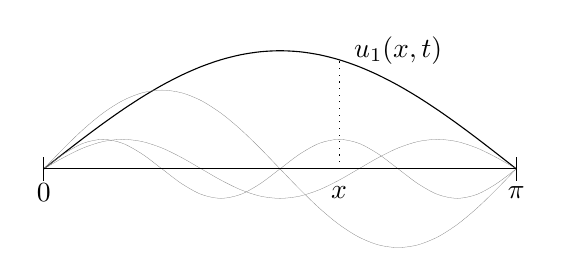
\begin{tikzpicture}[scale=3]
  \draw[domain=0:180, smooth] plot ({\x/90}, {1/2 * sin(\x)});
  \draw[gray, domain=0:180, smooth, ultra thin]
    plot ({\x/90}, {1/3 * sin(2*\x)});
  \draw[gray, domain=0:180, smooth, ultra thin]
    plot ({\x/90}, {1/8 * sin(3*\x)});
  \draw[gray, domain=0:180, smooth, ultra thin]
    plot ({\x/90}, {1/8 * sin(4*\x)});
  \draw (0, -0.05) -- (0, 0.05);
  \draw (2, -0.05) -- (2, 0.05);
  \draw (0, 0) -- (2, 0);
  \node at (0, -0.1) {$0$};
  \node at (2, -0.1) {$\pi$};
  \draw[dotted] (1.25, 0) -- (1.25, 0.463);

  \node at (1.5, 0.5) {$u_1(x, t)$};
  \node at (1.25, -0.1) {$x$};
\end{tikzpicture}
\end{document}
